\documentclass[diploma]{BMSTU-IU8}

\usepackage{todonotes}
\usepackage{lipsum}
\SetLipsumText{fishes}

\student{И. И. Иванов}
\theme{Создание отчёта \\ по НИРС \\ или ВКР}
\group{ИУ8-999}

\supervisor{П. П. Петров}
\researchConsultant{П. П. Петров}
\designConsultant{П. П. Петров}
\technologicalConsultant{П. П. Петров}
\economicsConsultant{П. П. Петров}
\lawsConsultant{П. П. Петров}
\normController{П. П. Петров}

% \theme{Тест \hfill} % Тема для НИРСа заполняется по-другому
\studentFullName{Иванов Иван Иванович}
\profile{10У101}
\speciality{10.05.01 <<Компьютерная безопасность>>}
\specialization{10.05.01\_01 <<Математические методы защиты информации>>}
\supervisorWithDegree{доцент, к.т.н. Иванов И. И.}

\newacronym{bd}{БД}{База данных.}
\newacronym{subd}{СУБД}{Система управления базами данных.}
\newacronym{cdc}{CDC}{Change Data Capture.}
\newacronym{gc}{GC}{Change Data Capture.}
\newacronym{ddl}{DDL}{Data Definition Language.}
\newacronym{dql}{DQL}{Data Query Language.}
\newacronym{dml}{DML}{Data Manipulation Language.}
\newacronym{dcl}{DCL}{Data Control Language.}
\newacronym{wal}{WAL}{Write-ahead log.}
\newacronym{lsn}{LSN}{Log sequence number.}
\newacronym{uri}{URI}{Uniform resource identifier.}
\newacronym{id}{ID}{Identifier.}
\newacronym{uuid}{UUID}{Universally unique identifier.}
\newacronym{ro}{RO}{Read-only.}
\newacronym{rw}{RW}{Read-write.}


\newglossaryentry{id7}{
    name={Анонимная реплика},
    description={это тип реплики, которая подключается к ведущему узлу для получения данных, но не участвует в кворуме репликации и не может стать мастером репликасета.}
}

\newglossaryentry{id1}{
    name={База данных (БД)},
    description={это организованная коллекция данных, которая структурирована таким образом, чтобы данные можно было легко хранить, управлять, изменять и извлекать.},
}

\newglossaryentry{id3}{
    name={Захват изменения данных (Change Data Capture, CDC)},
    description={это программное обеспечение для отслеживания и записи изменений, происходящих в данных базы данных. Оно позволяет фиксировать все вставки, обновления и удаления записей в режиме реального времени или с минимальной задержкой, что позволяет синхронизировать данные между различными системами, вести аудит изменений, и создавать системы резервного копирования или аналитики.}
}

\newglossaryentry{id6}{
    name={Кластер},
    description={это совокупность нескольких репликасетов, каждый из которых чаще всего хранит разный набор данных.}
}

\newglossaryentry{id10}{
    name={Локальный Спейс (local space)},
    description={это спейс, данные из которого не реплицируются и остаются локальными для конкретного узла.}
}

\newglossaryentry{id5}{
    name={Репликасет (replicaset)},
    description={это группа узлов (инстансов), работающих в режиме репликации и объединенных для обеспечения отказоустойчивости и доступности данных.}
}

\newglossaryentry{id2}{
    name={Система управления базами данных (СУБД)},
    description={это программное обеспечение, предназначенное для создания, управления и обеспечения доступа к базам данных. Оно позволяет пользователям определять, создавать, изменять и управлять базой данных, а также обеспечивает взаимодействие между пользователями и базой данных через запросы и команды. Основные функции включают хранение, поиск, обновление и удаление данных, а также обеспечение целостности, безопасности и управления доступом к данным.}
}

\newglossaryentry{id4}{
    name={Спейс (space)},
    description={это основная логическая единица хранения данных Tarantool, аналогичная таблице в традиционных реляционных базах данных. Спейс содержит набор записей, каждая из которых называется кортежем (tuple). Структура спейса определяется схемой, которая включает количество и типы полей в кортежах, а также индексы для быстрого доступа к данным.}
}

\newglossaryentry{id8}{
    name={LSN},
    description={это монотонно возрастающий идентификатор записи.}
}

\newglossaryentry{id9}{
    name={Vclock},
    description={это массив LSN, идентификаторами в котором являются ID узлов. Vclock представляет собой набор логических счетчиков для каждого узла в кластере, позволяя определить, какие изменения были применены на конкретном узле и какие еще предстоит синхронизировать.}
}


\addbibresource{main.bib}

\begin{document}
    % \maketitle
    % % \inlineimg{example.png}{\img}
    % \maketitle % Титульный лист

    % % \includepdf[pages=-]{extra/task} % Задание
    \setcounter{page}{4} % Устанавливает счётчик страниц

    \abstract

В данной работе рассматривается процесс настройки и управления репликацией в СУБД Tarantool, с акцентом на создание и конфигурацию репликасетов, подробно описывается процесс репликации и подключения узлов к репликасету. Работа также включает разработку дизайн-документа по фильтрации репликационного потока для улучшения работы Change Data Capture (CDC) в соответствии с требованиями заказчика.

 % Реферат

    \tableofcontents % Содержание
    % \termsanddefenitions % Термины и определения
    % \listofabbreviations % Перечень сокращений и обозначений

    \introduction

Место прохождения практики – общество с ограниченной ответственностью «ВК Цифровые Технологии», отдел Research \& Development, команда Tarantool Platform Core. Период прохождения практики - с 1 июля 2024 года по 28 июля 2024 года.

В задачи прохождения практики входило:

\begin{enumerate}
    \item Разобраться в работе асинхронной репликации СУБД Tarantool;
    \item Изучить протокол подключения новых реплик к существующему репликасету Tarantool;
    \item Разработать дизайн-документ по фильтрации репликационного потока.
\end{enumerate}

Основная цель прохождения практики заключалась в разработке дизайн-документа по фильтрации репликационного потока в СУБД Tarantool для улучшения работы CDC. От заказчика (команда разработки CDC) к новой функциональности были предъявлены следующие требования:

\begin{enumerate}
    \item Фильтрация репликационного потока по именам спейсов. Это необходимо для того, чтобы только выбранные спейсы передавались репликам, что обеспечивает более гибкое управление репликацией и снижает нагрузку на систему;
    \item Возможность продолжения подключения реплики к репликасету с места предыдущей остановки. Это позволяет уменьшить время восстановления работы реплик CDC после сбоев;
    \item Сохранение данных для анонимных реплик. Это необходимо, чтобы исключить ошибки репликации, связанные с удалением ненужных с точки зрения репликасета данных механизмом очистки (GC).
\end{enumerate}

Каждое из вышеуказанных требований направлено на улучшение работы кластерной системы Tarantool, обеспечивая высокую отказоустойчивость, масштабируемость и эффективность обработки данных в распределенной среде. Разработанный документ является основой для последующей реализации предложенных решений в коде и их интеграции в существующую архитектуру Tarantool.
 % Введение

    \structure{ОСНОВНАЯ~ЧАСТЬ}

\section{Маршрутизация}

В данной работе рассматривается использование широко распространённых open-source инструментов для реализации точечной маршрутизации по доменам. Основные компоненты данного метода — это dnsmasq и nftables.

Примером служит домен graylog.org, доступ к которому ограничен системой WAF Cloudflare для пользователей с российских IP-адресов. Это означает, что стандартное подключение к сайту через провайдера невозможно.

Процесс маршрутизации начинается с отправки компьютером DNS-запроса к маршрутизатору, чтобы разрешить доменное имя в IP-адрес \cite{tanenbaum}. В OpenWrt обработкой таких запросов занимается dnsmasq, обладающий функцией, позволяющей сопоставлять домены с IP-адресами и сохранять их в специальные таблицы (sets), поддерживаемые nftables.

Пример конфигурации представлен в листинге 1. Здесь list name задаёт таблицу (set), в которую будут записаны IP-адреса домена graylog.org. При запросе dnsmasq обращается к вышестоящему DNS-серверу, получает IP-адреса и возвращает их клиенту, одновременно добавляя их в указанный set (vpn\_domains).

\begin{lstlisting}[frame=rlbt,caption={Пример конфигурации Dnsmasq}]
config ipset
        list name 'vpn_domains'
        list domain 'graylog.org'
\end{lstlisting}

В дальнейшем, при поступлении пакета на маршрутизатор, если его IP-адрес совпадает с адресами из таблицы, маршрут определяет его направление через заранее настроенный туннель (например, VPN). Оставшийся трафик продолжает проходить через провайдера без изменений, что изображено на рисунке ~\ref{fig:fig01}.


\begin{figure}
  \centering
  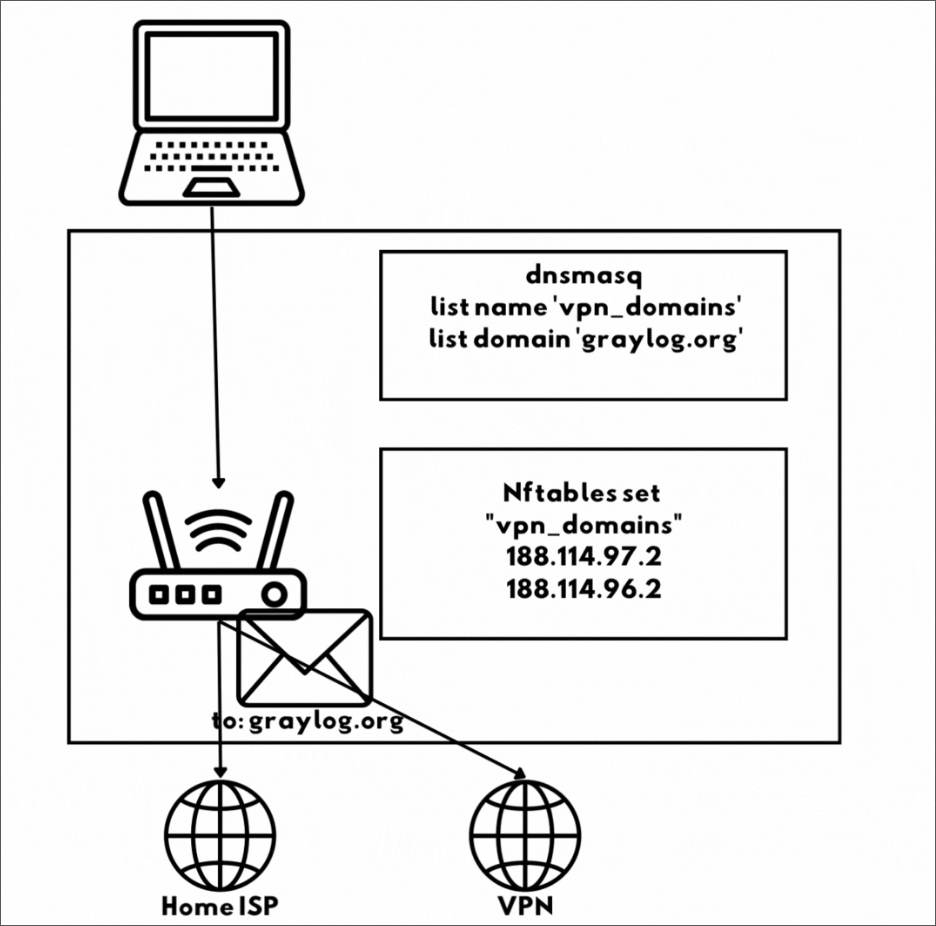
\includegraphics[scale=0.5]{inc/routing.png}
  \caption{Маршрутизация трафика}
  \label{fig:fig01}
\end{figure}

    \section{Настройка}

\subsection{Установка пакетов}

Для настройки точечной маршрутизации по доменам на OpenWrt требуется установка пакета dnsmasq-full, так как по умолчанию в прошивке используется урезанная версия dnsmasq для экономии места. Dnsmasq — это ключевой компонент системы, отвечающий за DNS-обслуживание, и его удаление может нарушить работу маршрутизатора. Поэтому перед установкой нового пакета необходимо выполнить несколько подготовительных шагов.

Процесс установки dnsmasq-full выглядит следующим образом \cite{openwrt}:

\begin{enumerate}
    \item Обновление индекса пакетов и скачивание dnsmasq-full. Для начала нужно обновить список доступных пакетов и выгрузить пакет dnsmasq-full в директорию /tmp:

\begin{lstlisting}[frame=rlbt]
opkg update && cd /tmp/ && opkg download dnsmasq-full
\end{lstlisting}

    \item Удаление стандартного dnsmasq. Поскольку стандартный dnsmasq не поддерживает необходимые функции, его нужно удалить перед установкой полной версии:

\begin{lstlisting}[frame=rlbt]
opkg remove dnsmasq
\end{lstlisting}

    \item Установка dnsmasq-full. Новый пакет устанавливается из кэша в директории /tmp. При этом важно сохранить текущие настройки DHCP, если они необходимы. Если файл /etc/config/dhcp имеет пользовательские изменения, стоит перенести конфигурацию вручную:

\begin{lstlisting}[frame=rlbt]
opkg install dnsmasq-full --cache /tmp/
mv /etc/config/dhcp-opkg /etc/config/dhcp
\end{lstlisting}

    \item Установка curl. Для работы со скриптами обновления списков доменов и проверки подключения потребуется установка утилиты curl:

\begin{lstlisting}[frame=rlbt]
    opkg install curl
\end{lstlisting}

\end{enumerate}

Эти шаги обеспечивают установку всех необходимых инструментов для реализации точечной маршрутизации по доменам на маршрутизаторе с OpenWrt

\subsection{Настройка маршрутизации}

Для управления трафиком и перенаправления его через VPN-туннель необходимо настроить специальную таблицу маршрутизации и правила для маркировки пакетов. Все пакеты с заданной маркировкой будут направляться в отдельную таблицу маршрутизации, которая перенаправляет трафик в туннель.

Добавляется новая таблица маршрутизации с уникальным идентификатором \cite{openwrt}:

\begin{lstlisting}[frame=rlbt]
echo '99 vpn' >> /etc/iproute2/rt_tables
\end{lstlisting}

Для указания, что весь трафик с определённой маркировкой должен использовать таблицу vpn, настраивается правило. Это можно выполнить через UCI или напрямую в конфигурационных файлах (/etc/config/network).

\begin{lstlisting}[frame=rlbt]
uci add network rule
uci set network.@rule[-1].name='mark0x1'
uci set network.@rule[-1].mark='0x1'
uci set network.@rule[-1].priority='100'
uci set network.@rule[-1].lookup='vpn'
uci commit network
\end{lstlisting}

Добавляется правило, направляющее весь трафик таблицы маршрутизации в туннель. В случае с WireGuard и интерфейсом wg0 выполняется следующая настройка.

\begin{lstlisting}[frame=rlbt]
uci set network.vpn_route=route
uci set network.vpn_route.interface='wg0'
uci set network.vpn_route.table='vpn'
uci set network.vpn_route.target='0.0.0.0/0'
uci commit network
\end{lstlisting}

Для туннелей, таких как OpenVPN, Sing-box, tun2socks, создающих интерфейсы типа device (например, tun0), настройка через UCI не поддерживается. В этом случае применяется hotplug. Создаётся файл /etc/hotplug.d/iface/30-vpnroute со следующим содержимым:

\begin{lstlisting}[frame=rlbt,language=bash]
#!/bin/sh

sleep 10
ip route add table vpn default dev tun0
\end{lstlisting}

\subsection{Настройка firewall}

Для обеспечения прохождения трафика через туннель требуется создать зону в файерволе, настроить nftables set для IP-адресов доменов, а также правило, которое будет маркировать трафик к этим адресам.

Зона для туннеля настраивается для обеспечения корректного прохождения трафика через него. Настройка зоны может варьироваться в зависимости от используемого туннеля (WireGuard, OpenVPN и т.д.) и описана в соответствующей документации для конкретного типа туннеля. Обычно создаётся зона с интерфейсом туннеля, например, wg0 или tun0, и задаются необходимые правила для передачи трафика между зонами.

Создаётся список vpn\_domains, в который будут автоматически добавляться IP-адреса доменов для точечной маршрутизации. Настройка через UCI выглядит следующим образом:

\begin{lstlisting}[frame=rlbt]
uci add firewall ipset
uci set firewall.@ipset[-1].name='vpn_domains'
uci set firewall.@ipset[-1].match='dst_net'
uci commit firewall
\end{lstlisting}

Для маркировки трафика, идущего к IP-адресам из списка vpn\_domains, создаётся правило:

\begin{lstlisting}[frame=rlbt]
uci add firewall rule
uci set firewall.@rule[-1]=rule
uci set firewall.@rule[-1].name='mark_domains'
uci set firewall.@rule[-1].src='lan'
uci set firewall.@rule[-1].dest='*'
uci set firewall.@rule[-1].proto='all'
uci set firewall.@rule[-1].ipset='vpn_domains'
uci set firewall.@rule[-1].set_mark='0x1'
uci set firewall.@rule[-1].target='MARK'
uci set firewall.@rule[-1].family='ipv4'
uci commit firewall
\end{lstlisting}

\subsection{Настройка автоматического обновления списка доменов}

Чтобы автоматически обновлять список доменов, которые необходимо перенаправлять
в тунель быд написан скрипт, включающий следующие функции:

\begin{itemize}
    \item Проверка доступности интернета после загрузки роутера.
    \item Загрузка готового конфигурационного файла в /tmp/dnsmasq.d/.
    \item Проверка валидности загруженного файла.
    \item Перезапуск службы dnsmasq при наличии корректной конфигурации.
\end{itemize}

Для обработки доменов и их резолвинга в списки IP-адресов используется конфигурация для dnsmasq. Она помещается в /tmp/dnsmasq.d/ — директорию для временных конфигураций. Пример конфигурации:

\begin{lstlisting}[frame=rlbt]
nftset=/graylog.org/4#inet#fw4#vpn_domains
nftset=/terraform.io/4#inet#fw4#vpn_domains
\end{lstlisting}

Каждая строка добавляет домен (включая субдомены) в список vpn\_domains. Таким образом, IP-адреса доменов автоматически помещаются в таблицу маршрутизации.

Скрипт обновления списка доменов (/etc/init.d/getdomains):

\begin{lstlisting}[frame=rlbt,language=bash]
#!/bin/sh /etc/rc.common

START=99

start () {
    DOMAINS=https://raw.githubusercontent.com/itdoginfo/allow-domains/main/Russia/inside-dnsmasq-nfset.lst

    count=0
    while true; do
        if curl -m 3 github.com; then
            curl -f $DOMAINS --output /tmp/dnsmasq.d/domains.lst
            break
        else
            echo "GitHub is not available. Check the internet availability [$count]"
            count=$((count+1))
        fi
    done

    if dnsmasq --conf-file=/tmp/dnsmasq.d/domains.lst --test 2>&1 | grep -q "syntax check OK"; then
        /etc/init.d/dnsmasq restart
    fi
}
\end{lstlisting}

Скрипт необходимо сделать исполняемым и добавить в автозагрузку:

\begin{lstlisting}[frame=rlbt]
chmod +x /etc/init.d/getdomains
ln -sf ../init.d/getdomains /etc/rc.d/S99getdomains
\end{lstlisting}

Для регулярного обновления конфигурации используется cron. Добавляется задание на обновление списка каждые 8 часов \cite{cron}. В файл crontab добавляется строка:

\begin{lstlisting}[frame=rlbt]
0 */8 * * * /etc/init.d/getdomains start
\end{lstlisting}

После настройки выполняется перезапуск сети и ручной запуск скрипта:

\begin{lstlisting}[frame=rlbt]
service network restart
service getdomains start
\end{lstlisting}

Преимущества подхода:

\begin{itemize}
    \item Ускорение работы: Готовые конфигурации избавляют от необходимости конвертировать списки вручную.
    \item Удобство обновления: Скрипт автоматически загружает и проверяет новые списки.
    \item Автоматизация: Настройка автозапуска и периодического обновления обеспечивает бесперебойную работу маршрутизации.
\end{itemize}

\subsection{Добавление доменов в обход скрипта}

Для добавления необходимых доменов в список vpn\_domains через конфигурацию dnsmasq требуется изменить файл /etc/config/dhcp. В конце файла добавляется следующий блок:

\begin{lstlisting}[frame=rlbt]
config ipset
        list name 'vpn_domains'
        list domain 'graylog.org'
        list domain 'terraform.io'
\end{lstlisting}

Каждый домен добавляется новой строкой с ключевым словом list domain. Поскольку dnsmasq поддерживает wildcard, добавлять субдомены отдельно не требуется — они автоматически обрабатываются. После внесения изменений для применения настроек необходимо перезапустить dnsmasq:

\begin{lstlisting}[frame=rlbt]
service dnsmasq restart
\end{lstlisting}

\subsection{Возможные проблемы}

В случае точечной маршрутизации через домены на роутере с OpenWrt могут возникнуть проблемы, если провайдер вмешивается в DNS-запросы или блокирует трафик, что нарушает корректную работу маршрутизации. Существуют несколько возможных ситуаций:

\begin{enumerate}
    \item Подмена IP-адресов на DNS-серверах провайдера. В этом случае достаточно просто сменить DNS-сервер на роутере (например, на 8.8.8.8 или 8.8.4.4), чтобы обойти эту подмену.

    \item Провайдер подменяет запросы на своих DNS-серверах, даже если использовать другие DNS-серверы (например, 8.8.8.8), оборудование провайдера может перехватывать и изменять DNS-запросы. Для решения этой проблемы можно настроить DNS over TLS или DNS over HTTPS.

    \item Провайдер блокирует весь трафик на порту 53, кроме запросов к своим DNS-серверам. В этой ситуации необходимо использовать зашифрованные каналы для DNS-запросов, такие как DNS over TLS или DNS over HTTPS.
\end{enumerate}

Для обхода блокировки DNS-запросов можно установить один из двух популярных резолверов, поддерживающих шифрование: DNSCrypt-proxy2 или Stubby. Если на роутере ограниченное количество памяти, например, 16 МБ, лучше выбрать Stubby из-за его меньшего размера. В остальных случаях можно использовать DNSCrypt для более широких возможностей.

\subsubsection*{DNSCrypt-proxy2}

DNSCrypt-proxy2 позволяет шифровать DNS-запросы через DNS over TLS или DNS over HTTPS. Этот инструмент требует больше места на роутере (около 10.7 МБ), но предоставляет расширенные функции \cite{dnscrypt}.

\begin{lstlisting}[frame=rlbt]
opkg update && opkg install dnscrypt-proxy2
\end{lstlisting}

Конфигурация изменяется в файле /etc/dnscrypt-proxy2/dnscrypt-proxy.toml, где можно выбрать серверы в параметре server\_names. После этого нужно перезапустить сервис:

\begin{lstlisting}[frame=rlbt]
service dnscrypt-proxy restart
\end{lstlisting}

Далее настраиваем dnsmasq, чтобы он использовал DNSCrypt как сервер:

\begin{lstlisting}[frame=rlbt]
uci set dhcp.@dnsmasq[0].noresolv="1"
uci -q delete dhcp.@dnsmasq[0].server
uci add_list dhcp.@dnsmasq[0].server="127.0.0.53#53"
uci commit dhcp
service dnsmasq restart
\end{lstlisting}

Теперь все DNS-запросы будут шифроваться через DNSCrypt.

\subsubsection*{Stubby}

Stubby — это более легковесная альтернатива DNSCrypt, занимающая всего 36K + библиотеки. Он использует DNS over TLS и по умолчанию настроен на сервера Cloudflare.

\begin{lstlisting}[frame=rlbt]
opkg update && opkg install stubby
\end{lstlisting}

Конфигурация по умолчанию использует 127.0.0.1:5453, но можно настроить другие серверы в /etc/config/stubby. Для настройки dnsmasq нужно изменить сервер на 127.0.0.1\#5453:

\begin{lstlisting}[frame=rlbt]
uci set dhcp.@dnsmasq[0].noresolv="1"
uci -q delete dhcp.@dnsmasq[0].server
uci add_list dhcp.@dnsmasq[0].server="127.0.0.1#5453"
uci commit dhcp
service dnsmasq restart
\end{lstlisting}

    \section{Автоматическая настройка}

Для автоматизации настроек точечной маршрутизации на роутере с OpenWrt, был создан скрипт, который выполняет шаги, описанные в предыдущей части. Полный код скрипта представлен в Приложении 1. Скрипт предполагает свежую установку OpenWrt или минимальные изменения в текущей конфигурации. Если на роутере уже есть другие туннели или маршруты, выполнение скрипта может привести к некорректной настройке, поэтому рекомендуется предварительно проверить текущую конфигурацию.

\begin{enumerate}
    \item Выбор туннеля: Скрипт предложит выбрать туннель. Для WireGuard (WG) настройка будет выполнена автоматически. Для OpenVPN, sing-box или tun2socks потребуется вручную настроить соответствующие клиенты. Для sing-box скрипт создаст шаблон конфигурации.
    \item Подмена DNS-запросов: Если провайдер подменяет DNS-запросы, скрипт предложит установить резолверы, такие как DNSCrypt-proxy2 или Stubby. DNSCrypt-proxy2 более функционален, но занимает больше памяти, в то время как Stubby более легковесен.
    \item Выбор доменов: Скрипт позволяет легко выбрать список доменов, для которых будет настроена точечная маршрутизация. Эти списки загружаются автоматически и добавляются в конфигурацию DNS-сервера.
    \item Смена туннелей: Скрипт также позволяет легко переключать туннели. Например, при переходе с OpenVPN на sing-box он автоматически обновит файрвол, но для предотвращения конфликтов интерфейсов потребуется вручную остановить старую службу или изменить интерфейс.
\end{enumerate}

Этот скрипт значительно упрощает настройку, но в сложных случаях, когда требуются изменения в существующих туннелях или маршрутах, может потребоваться ручное вмешательство.



    \conclusion

Таким образом, в ходе прохождения практики был разработан новый протокол подключения анонимных реплик, удовлетворяющий требованиям команды CDC. Он выглядит следующим образом:

\begin{enumerate}
    \item Анонимая реплика отправляет IPROTO\_FETCH\_SNAPSHOT, сообщая мастеру, что она хочет реплицироваться с него. В этот запрос может быть включены следующие опции:
    \begin{enumerate}
        \item IPROTO\_CURSOR - реплика хочет использовать файловый JOIN для возможности продолжения подключения в случае разрыва подключения.
        \item IPROTO\_IS\_PERSISTENT\_GC - необходимо создать анонимного GC consumer и сохранять xlog файлы для данной реплики.
        \item IPROTO\_SPACE\_NAME\_FILTER - поток репликации должен быть фильтрованным. Требуются только частичные данные.
    \end{enumerate}
    \item В ответ мастер посылает vclock read-view или файла снапшота (в зависимости от IPROTO\_CURSOR). Мастер создает анонимный GC consumer, если опция IPROTO\_IS\_PERSISTENT\_GC равен true.
    \item Мастер начинает пересылку данных. Если IPROTO\_SPACE\_NAME\_FILTER указан, то данные фильтруются на стороне сервера и посылаются частично.
    \item Реплика посылает IPROTO\_SUBSCRIBE, указывая необходимость GC consumer и фильтрации потока.
\end{enumerate}

В любой момент времени процесс подключения может быть разорван и продолжен с того же момента. Ошибки удаления файлов xlog больше не возникают, так как теперь есть возможность их сохранения для анонимных реплик. Нагрузка на CDC реплики была снижена, так как теперь им больше не приходится самостоятельно обрабатывать фильтрацию репликации.


    \printbibliography

    \appendix
    \appendixsection{Спецификация Raft на TLA+}

\end{document}
